W każdym momencie procesor działa albo w trybie użytkownika, albo w trybie uprzywilejowanym. W trybie uprzywilejowanym dostępne są instrukcje dające pełną kontrolę nad komputerem, a w trybie użytkownika dostęp ten jest ograniczony.

\begin{figure}[H]  
    \centering
    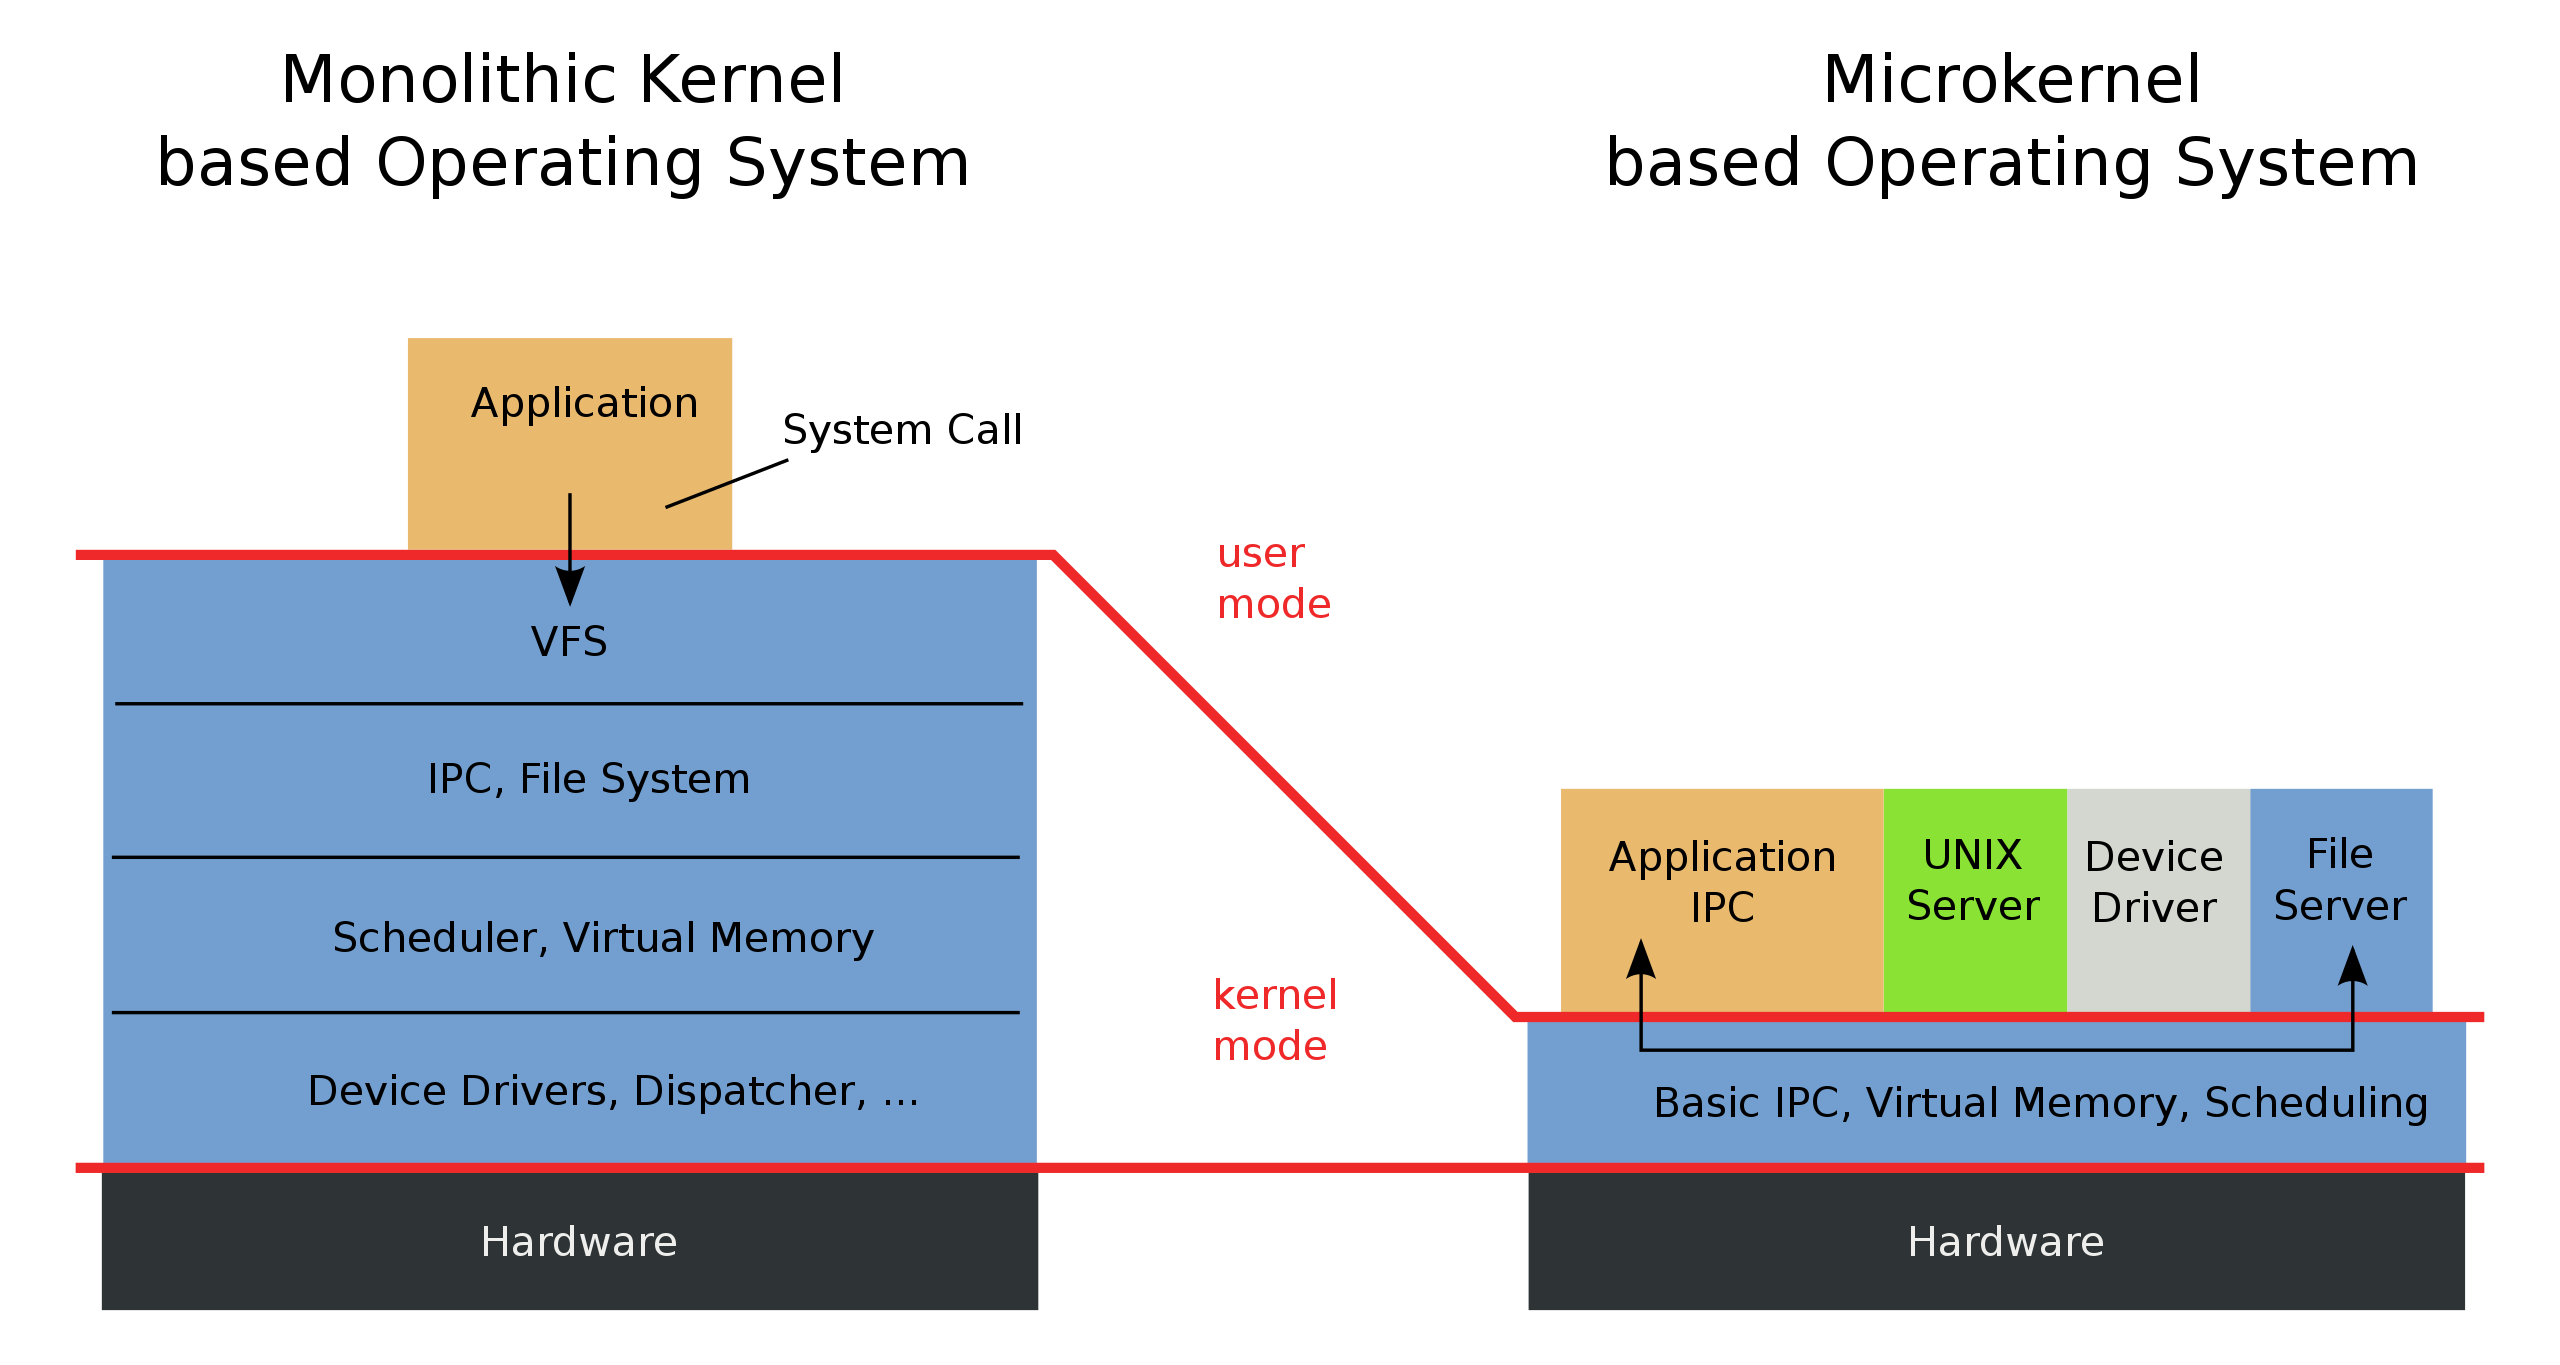
\includegraphics[width=12cm]{chapters/sysopy/monolit/os-structure}
\caption{Public domain, Wikimedia Commons; Model komunikacji z aplikacjami monolitu i mikro jądra}
\end{figure}

\subsection{Monolit}
W monolitycznej architekturze cały system operacyjny działa w trybie uprzywilejowanym. W szczególności, wszystkie sterowniki urządzeń działają w trybie uprzywilejowanym, więc usterka w dowolnym z nich zaburza działanie całego systemu operacyjnego. Proces użytkownika wykonuje żądanie systemowe poprzez bezpośrednie przejście do trybu uprzywilejowanego, w którym odpowiedni kod kernela obsługuje to żądanie.

\subsection{Mikro jądro}
W architekturze opartej na mikro jądrze minimalizuje się ilość kodu było wykonywanego w trybie uprzywilejowanym. Wiele zadań systemu operacyjnego, takie jak zarządzanie procesami czy obsługa systemów plików jest wykonywana przez serwery, czyli specjalne procesy, które działają w trybie użytkownika, ale mogą prosić kernel o wykonywanie dla nich odpowiednich operacji. W szczególności sterowniki urządzeń są zwykłymi serwerami. Dzięki podziale zadań na różne serwery, cały system operacyjny staje się bardziej modularny, a usterka w pojedynczym serwerze niekoniecznie zaburza działania całego systemu. Procesy użytkownika, podobnie jak serwery, nigdy nie działają w trybie uprzywilejowanym. Wykonują żądania systemowe, przekazując wiadomości do odpowiednich serwerów, które realizują je, przekazując odpowiednie wiadomości dalej do kernela. Tylko kernel działa w trybie uprzywilejowanym i musi być odpowiedzialny przynajmniej za komunikację między procesami, mapowanie wirtualnej pamięci, przełączanie procesów oraz bezpośrednią komunikację z urządzeniami.